\documentclass{ximera}

%\usepackage{todonotes}

\newcommand{\todo}{}

\usepackage{tkz-euclide}
\tikzset{>=stealth} %% cool arrow head
\tikzset{shorten <>/.style={ shorten >=#1, shorten <=#1 } } %% allows shorter vectors

\usepackage{tkz-tab}  %% sign charts
\usetikzlibrary{decorations.pathreplacing} 

\usetikzlibrary{backgrounds} %% for boxes around graphs
\usetikzlibrary{shapes,positioning}  %% Clouds and stars
\usetikzlibrary{matrix} %% for matrix
\usepgfplotslibrary{polar} %% for polar plots
\usetkzobj{all}
\usepackage[makeroom]{cancel} %% for strike outs
%\usepackage{mathtools} %% for pretty underbrace % Breaks Ximera
\usepackage{multicol}

\usepackage{polynom}



\usepackage[many]{tcolorbox}  %% for titled boxes
\newtcolorbox{xbox}[1]{%
    tikznode boxed title,
    enhanced,
    arc=0mm,
    interior style={white},
    attach boxed title to top center= {yshift=-\tcboxedtitleheight/2},
    fonttitle=\bfseries,
    colbacktitle=white,coltitle=black,
    boxed title style={size=normal,colframe=white,boxrule=0pt},
    title={#1}}


\usepackage{array}
\setlength{\extrarowheight}{+.1cm}   
\newdimen\digitwidth
\settowidth\digitwidth{9}
\def\divrule#1#2{
\noalign{\moveright#1\digitwidth
\vbox{\hrule width#2\digitwidth}}}





\newcommand{\RR}{\mathbb R}
\newcommand{\R}{\mathbb R}
\newcommand{\N}{\mathbb N}
\newcommand{\Z}{\mathbb Z}

%\renewcommand{\d}{\,d\!}
\renewcommand{\d}{\mathop{}\!d}
\newcommand{\dd}[2][]{\frac{\d #1}{\d #2}}
\newcommand{\pp}[2][]{\frac{\partial #1}{\partial #2}}
\renewcommand{\l}{\ell}
\newcommand{\ddx}{\frac{d}{\d x}}
\newcommand{\ddt}{\frac{d}{\d t}}

\newcommand{\zeroOverZero}{\ensuremath{\boldsymbol{\tfrac{0}{0}}}}
\newcommand{\inftyOverInfty}{\ensuremath{\boldsymbol{\tfrac{\infty}{\infty}}}}
\newcommand{\zeroOverInfty}{\ensuremath{\boldsymbol{\tfrac{0}{\infty}}}}
\newcommand{\zeroTimesInfty}{\ensuremath{\small\boldsymbol{0\cdot \infty}}}
\newcommand{\inftyMinusInfty}{\ensuremath{\small\boldsymbol{\infty - \infty}}}
\newcommand{\oneToInfty}{\ensuremath{\boldsymbol{1^\infty}}}
\newcommand{\zeroToZero}{\ensuremath{\boldsymbol{0^0}}}
\newcommand{\inftyToZero}{\ensuremath{\boldsymbol{\infty^0}}}



\newcommand{\numOverZero}{\ensuremath{\boldsymbol{\tfrac{\#}{0}}}}
\newcommand{\dfn}{\textbf}
%\newcommand{\unit}{\,\mathrm}
\newcommand{\unit}{\mathop{}\!\mathrm}
\newcommand{\eval}[1]{\bigg[ #1 \bigg]}
\newcommand{\seq}[1]{\left( #1 \right)}
\renewcommand{\epsilon}{\varepsilon}
\renewcommand{\iff}{\Leftrightarrow}

\DeclareMathOperator{\arccot}{arccot}
\DeclareMathOperator{\arcsec}{arcsec}
\DeclareMathOperator{\arccsc}{arccsc}
\DeclareMathOperator{\si}{Si}
\DeclareMathOperator{\proj}{proj}
\DeclareMathOperator{\scal}{scal}


\newcommand{\tightoverset}[2]{% for arrow vec
  \mathop{#2}\limits^{\vbox to -.5ex{\kern-0.75ex\hbox{$#1$}\vss}}}
\newcommand{\arrowvec}[1]{\tightoverset{\scriptstyle\rightharpoonup}{#1}}
\renewcommand{\vec}{\mathbf}
\newcommand{\veci}{\vec{i}}
\newcommand{\vecj}{\vec{j}}
\newcommand{\veck}{\vec{k}}
\newcommand{\vecl}{\boldsymbol{\l}}

\newcommand{\dotp}{\bullet}
\newcommand{\cross}{\boldsymbol\times}
\newcommand{\grad}{\boldsymbol\nabla}
\newcommand{\divergence}{\grad\dotp}
\newcommand{\curl}{\grad\cross}
%\DeclareMathOperator{\divergence}{divergence}
%\DeclareMathOperator{\curl}[1]{\grad\cross #1}


\colorlet{textColor}{black} 
\colorlet{background}{white}
\colorlet{penColor}{blue!50!black} % Color of a curve in a plot
\colorlet{penColor2}{red!50!black}% Color of a curve in a plot
\colorlet{penColor3}{red!50!blue} % Color of a curve in a plot
\colorlet{penColor4}{green!50!black} % Color of a curve in a plot
\colorlet{penColor5}{orange!80!black} % Color of a curve in a plot
\colorlet{fill1}{penColor!20} % Color of fill in a plot
\colorlet{fill2}{penColor2!20} % Color of fill in a plot
\colorlet{fillp}{fill1} % Color of positive area
\colorlet{filln}{penColor2!20} % Color of negative area
\colorlet{fill3}{penColor3!20} % Fill
\colorlet{fill4}{penColor4!20} % Fill
\colorlet{fill5}{penColor5!20} % Fill
\colorlet{gridColor}{gray!50} % Color of grid in a plot

\newcommand{\surfaceColor}{violet}
\newcommand{\surfaceColorTwo}{redyellow}
\newcommand{\sliceColor}{greenyellow}




\pgfmathdeclarefunction{gauss}{2}{% gives gaussian
  \pgfmathparse{1/(#2*sqrt(2*pi))*exp(-((x-#1)^2)/(2*#2^2))}%
}


%%%%%%%%%%%%%
%% Vectors
%%%%%%%%%%%%%

%% Simple horiz vectors
\renewcommand{\vector}[1]{\left\langle #1\right\rangle}


%% %% Complex Horiz Vectors with angle brackets
%% \makeatletter
%% \renewcommand{\vector}[2][ , ]{\left\langle%
%%   \def\nextitem{\def\nextitem{#1}}%
%%   \@for \el:=#2\do{\nextitem\el}\right\rangle%
%% }
%% \makeatother

%% %% Vertical Vectors
%% \def\vector#1{\begin{bmatrix}\vecListA#1,,\end{bmatrix}}
%% \def\vecListA#1,{\if,#1,\else #1\cr \expandafter \vecListA \fi}

%%%%%%%%%%%%%
%% End of vectors
%%%%%%%%%%%%%

%\newcommand{\fullwidth}{}
%\newcommand{\normalwidth}{}



%% makes a snazzy t-chart for evaluating functions
%\newenvironment{tchart}{\rowcolors{2}{}{background!90!textColor}\array}{\endarray}

%%This is to help with formatting on future title pages.
\newenvironment{sectionOutcomes}{}{} 



%% Flowchart stuff
%\tikzstyle{startstop} = [rectangle, rounded corners, minimum width=3cm, minimum height=1cm,text centered, draw=black]
%\tikzstyle{question} = [rectangle, minimum width=3cm, minimum height=1cm, text centered, draw=black]
%\tikzstyle{decision} = [trapezium, trapezium left angle=70, trapezium right angle=110, minimum width=3cm, minimum height=1cm, text centered, draw=black]
%\tikzstyle{question} = [rectangle, rounded corners, minimum width=3cm, minimum height=1cm,text centered, draw=black]
%\tikzstyle{process} = [rectangle, minimum width=3cm, minimum height=1cm, text centered, draw=black]
%\tikzstyle{decision} = [trapezium, trapezium left angle=70, trapezium right angle=110, minimum width=3cm, minimum height=1cm, text centered, draw=black]


\outcome{Know the properties of rational functions.}
\outcome{Understand the definition of a rational function.}

\title[Dig-In:]{Graphs of rational functions}


\begin{document}
\begin{abstract}
	Rough graphs of rational functions
\end{abstract}
\maketitle


\section{Graphing rational functions}


There is a somewhat wide variation in the graphs of rational
functions.

\begin{example}
    Here we see the the graphs of four rational functions.
\begin{image}
  \begin{tabular}{cc}
    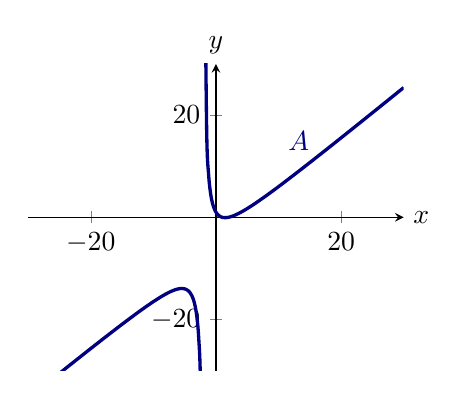
\begin{tikzpicture}
      \begin{axis}[
          xmin=-30,xmax=30,
            ymin=-30,ymax=30,
            domain=-2:2,
            width=2.5in,
            axis lines =middle, xlabel=$x$, ylabel=$y$,
            every axis y label/.style={at=(current axis.above origin),anchor=south},
            every axis x label/.style={at=(current axis.right of origin),anchor=west},
        ]
	\addplot [very thick, penColor, smooth, samples=100, domain=-30:-2.2] {(x^2-3*x+2)/(x+2)};
       	\addplot [very thick, penColor, smooth, samples=100, domain=-1.8:30] {(x^2-3*x+2)/(x+2)};

        \node at (axis cs:10,15) [penColor,anchor=west] {$A$};          
      \end{axis}
    \end{tikzpicture}
    &
    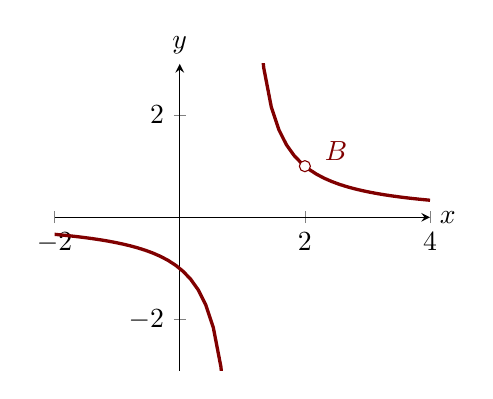
\begin{tikzpicture}
	\begin{axis}[
            xmin=-2,xmax=4,
            ymin=-3,ymax=3,
            width=2.5in,
            axis lines =middle, xlabel=$x$, ylabel=$y$,
            every axis y label/.style={at=(current axis.above origin),anchor=south},
            every axis x label/.style={at=(current axis.right of origin),anchor=west},
          ]
	  \addplot [very thick, penColor2, domain=-2:.9] {1/(x-1)};
          \addplot [very thick, penColor2, domain=1.1:4] {1/(x-1)};
          \addplot[color=penColor2,fill=background,only marks,mark=*] coordinates{(2,1)};  %% open hole
          \node at (axis cs:2.5,1.3) [penColor2] {$B$};
        \end{axis}
    \end{tikzpicture}
        \\
    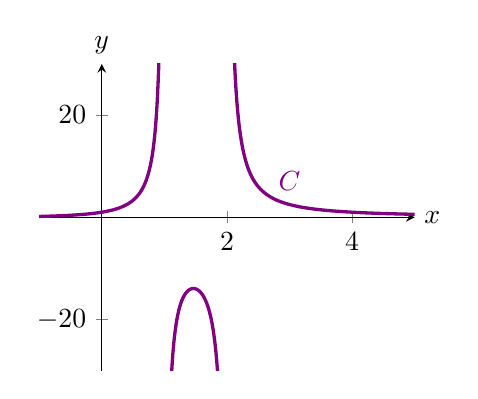
\begin{tikzpicture}
      \begin{axis}[
          xmin=-1,xmax=5,
          ymin=-30,ymax=30,
          width=2.5in,
          axis lines =middle, xlabel=$x$, ylabel=$y$,
          every axis y label/.style={at=(current axis.above origin),anchor=south},
          every axis x label/.style={at=(current axis.right of origin),anchor=west},
        ]
        \addplot [very thick, penColor3, smooth, samples=100, domain=-1:.95] {(x+2)/(x^2-3*x+2)};
        \addplot [very thick, penColor3, smooth, samples=100, domain=1.1:1.9]  {(x+2)/(x^2-3*x+2)};
        \addplot [very thick, penColor3, smooth, samples=100, domain=2.1:5]  {(x+2)/(x^2-3*x+2)};
        \node at (axis cs:3,7) [penColor3] {$C$};
      \end{axis}
    \end{tikzpicture}
    &
 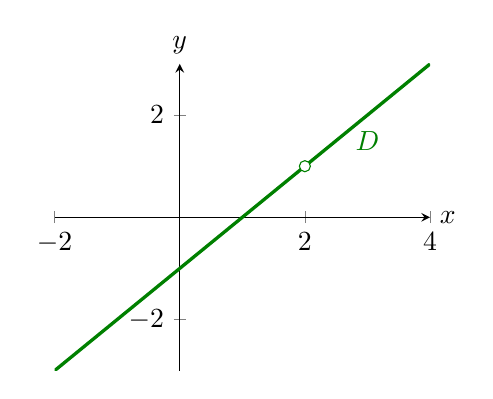
\begin{tikzpicture}
      \begin{axis}[
          xmin=-2,xmax=4,
          ymin=-3,ymax=3,
          domain=-2:4,
          width=2.5in,
          axis lines =middle, xlabel=$x$, ylabel=$y$,
          every axis y label/.style={at=(current axis.above origin),anchor=south},
          every axis x label/.style={at=(current axis.right of origin),anchor=west},
        ]
	\addplot [very thick, penColor4] {x-1};
        \addplot[color=penColor4,fill=background,only marks,mark=*] coordinates{(2,1)};  %% open hole
        \node at (axis cs:3,1.5) [penColor4] {$D$};
      \end{axis}
    \end{tikzpicture}
  \end{tabular}
\end{image}
Match the curves $A$, $B$, $C$, and $D$ with the functions
  \begin{align*}
    &\frac{x^2-3x+2}{x-2}, &&\frac{x^2-3x+2}{x+2}, \\
    &\frac{x-2}{x^2-3x+2}, &&\frac{x+2}{x^2-3x+2}.
  \end{align*}
\begin{explanation}
  Consider $\frac{x^2-3x+2}{x-2}$. This function is undefined only at
  $x=2$. Of the curves that we see above, $\answer[given]{D}$ is
  undefined exactly at $x=2$.

  Now consider $\frac{x^2-3x+2}{x+2}$. This function is undefined only
  at $x=-2$. The only function above that undefined exactly at $x=-2$
  is curve $\answer[given]{A}$.

  Now consider $\frac{x-2}{x^2-3x+2}$. This function is undefined at
  the roots of
  \[
  x^2-3x+2 = (x-2)(x-1).
  \]
  Hence it is undefined at $x=2$ and $x=1$. It looks like both curves
  $B$ and $C$ would work. Distinguishing between these two curves is
  easy enough if we evaluate at $x=-2$. Check it out.
  \begin{align*}
    \eval{\frac{x-2}{x^2-3x+2}}_{x=-2} &= \frac{-2-2}{(-2)^2-3(-2)+2}\\
    &= \frac{-4}{4+6+2}\\
    &=\frac{-4}{12}.
  \end{align*}
  Since this is negative, we see that $\frac{x-2}{x^2-3x+2}$
  corresponds to curve $\answer[given]{B}$.

  Finally, it must be the case that curve $\answer[given]{C}$
  corresponds to $\frac{x+2}{x^2-3x+2}$. We should note that if this
  function is evaluated at $x=-2$, the output is zero, and this
  corroborates our work above.
\end{explanation}
\end{example}


\end{document}
